\documentclass[conference]{IEEEtran}

%\IEEEoverridecommandlockouts
% The preceding line is only needed to identify funding in the first footnote. If that is unneeded, please comment it out.

\usepackage{cite}
\usepackage{amsmath,amssymb,amsfonts}
\usepackage{algorithmic}
\usepackage{graphicx}
\usepackage{textcomp}
\usepackage{xcolor}
\usepackage[]{hyperref}
\usepackage{subfigure}
\usepackage{booktabs}

\graphicspath{{./figures/}}

%\def\BibTeX{{\rm B\kern-.05em{\sc i\kern-.025em b}\kern-.08em
%    T\kern-.1667em\lower.7ex\hbox{E}\kern-.125emX}}
\newcommand{\cheng}[1]{{\textcolor{red}{ #1}}}
% correct bad hyphenation here
\hyphenation{}



\begin{document}

% paper title
% Titles are generally capitalized except for words such as a, an, and, as,
% at, but, by, for, in, nor, of, on, or, the, to and up, which are usually
% not capitalized unless they are the first or last word of the title.
% Linebreaks \\ can be used within to get better formatting as desired.
% Do not put math or special symbols in the title.
\title{Persistent Fault Analysis of Convolutional Neural Networks on FPGA-based Acceleration System}

% author info
%\author{\IEEEauthorblockN{1\textsuperscript{st} Given Name Surname}
%\IEEEauthorblockA{\textit{dept. name of organization (of Aff.)} \\
%\textit{name of organization (of Aff.)}\\
%City, Country \\
%email address}
%\and
%\IEEEauthorblockN{2\textsuperscript{nd} Given Name Surname}
%\IEEEauthorblockA{\textit{dept. name of organization (of Aff.)} \\
%\textit{name of organization (of Aff.)}\\
%City, Country \\
%email address}
%\and
%\IEEEauthorblockN{3\textsuperscript{rd} Given Name Surname}
%\IEEEauthorblockA{\textit{dept. name of organization (of Aff.)} \\
%\textit{name of organization (of Aff.)}\\
%City, Country \\
%email address}
%\and
%\IEEEauthorblockN{4\textsuperscript{th} Given Name Surname}
%\IEEEauthorblockA{\textit{dept. name of organization (of Aff.)} \\
%\textit{name of organization (of Aff.)}\\
%City, Country \\
%email address}
%\and
%\IEEEauthorblockN{5\textsuperscript{th} Given Name Surname}
%\IEEEauthorblockA{\textit{dept. name of organization (of Aff.)} \\
%\textit{name of organization (of Aff.)}\\
%City, Country \\
%email address}
%\and
%\IEEEauthorblockN{6\textsuperscript{th} Given Name Surname}
%\IEEEauthorblockA{\textit{dept. name of organization (of Aff.)} \\
%\textit{name of organization (of Aff.)}\\
%City, Country \\
%email address}
%}

% make the title area
\maketitle


% As a general rule, do not put math, special symbols or citations
% in the abstract
\begin{abstract}
    Deep neural network (DNN) is making continuous breakthroughs 
    in massive domains of applications and is increasingly 
    deployed on customized DNN accelerators for both the 
    higher performance and energy efficiency. While the 
    increasing hardware failures caused by the shrinking semiconductor 
    technology may have substantial influence on the accelerators and 
    improving the resilience of the neural network execution becomes a great 
    challenge especially to mission-critical applications such as self-driving 
    and medical diagnose. The reliability analysis of the neural 
    network execution is a key step to understand and alleviate the influence 
    of the hardware failures, and thus is highly demanded. 
    
    Prior works typically focus on the computing errors of neural networks caused by 
    hardware faults with simulation, but there is still a lack of fault 
    analysis from a system point of view. For instance, the consequences of 
    the system such as system stall are also critical to resilient 
    neural network execution. In this work, we implemented a 
    representative neural network accelerator as well as fault injection modules 
    on a Xilinx ARM-FPGA platform (ZC706). Then we conducted comprehensive fault 
    analysis of the system using four typical neural network models
    from different system angles including system functionality, 
    fault coverage, and input variation as well as prediction 
    accuracy loss. Based on the analysis, we find that system stall 
    caused by hardware faults is non-trivial to the system reliability 
    and further propose an efficient approach to alleviate it with negligible 
    hardware overhead. 
    
\end{abstract}


%\begin{IEEEkeywords}
    % keyword1, keyword2, keyword3, keyword4, keyword5
%\end{IEEEkeywords}


% For peer review papers, you can put extra information on the cover
% page as needed:
% \ifCLASSOPTIONpeerreview
% \begin{center} \bfseries EDICS Category: 3-BBND \end{center}
% \fi
%
% For peerreview papers, this IEEEtran command inserts a page break and
% creates the second title. It will be ignored for other modes.
\IEEEpeerreviewmaketitle

\section{Introduction}
Improving general-purpose processing system is getting extremely 
difficult. More and more computer architects believe that the major 
improvements in cost-energy-performance will come from domain-specific 
hardware accelerators. Recent years have already seen a number of successful 
demonstrations utilizing domain specific hardware accelerators for critical 
domains of applications such as deep neural network \cite{Jouppi2017tpu, Li2017survey} 
database operations \cite{Wu2014q100} and graph processing \cite{Jun2016graphicionado, Ozdal2016energy}. 
In order to explore the hardware accelerator design, a hardware accelerator simulator 
is usually required. Indeed there are already many exisitng tools \cite{systemc, chisel} and 
models \cite{dramsim2, ramulator} that can be used to help with the hardware accelerator 
design, it is non-trivial to develop a hardware accelerator on top of these work. For instance, there 
is a lack of general public cycle-accurate memory models available in \cite{systemc, chisel} while 
\cite{dramsim2, ramulator} expose only primitive memory access interface and need to be further 
wrapped for an accelerator simulator. And a general accelerator simulator 
framework is highly desired for the hardware accelerator simulator development.

Despite the difference of the accelerator simulators, we argue that a general 
accelerator simulator design framework should have three common yet important 
features. First of all, it should provide memory models of various memory 
architectures. Basically memory is usually critical to the hardware accelerator 
and greatly affects the accelerator design. At the same time, memory techniques evolve rapidly 
over the years and novel memory architectures with distinct features emerge. In order to explore 
hardware accelerator design, various memory architectures needs to be evaluated. 
Secondly, it should provide abstract user-frinedly memory interfaces. Hardware accelerators 
usually have complex memory access patterns such as stream access, burst access as well as random access. 
Thus higher abstract memory access interface instead of primitive memory access interface should be provided. 
Thirdly, it should provide trade-off between simulation speed and precision. Hardware accelerators 
may have distinct simulation speed and precision requirements while exploring the hardware accelerator. 
For instance, some of the applications such as graph accelerators may process on a big data set. 
Low-level accurate memory model may result in extremely long simulation. Thus a simplified memory model 
should be used to obtain the general performance of the accelerators. For applications that are sensitive 
to the memory access latency, more accurate memory models are preferred.

There is still a lack of general accelerator simulator framework that fullfills 
all the three features mentioned above. To that end, we proposed a flexible hardware accelerator 
simulation framework to be reused for general hardware accelerator simulator development. Basically, it 
integrates ramulator supporting various memory architectures as the underlying memory model and thus allows 
hardware accelerator exploration over a broad range of memory architectures. In addition, abstract memory 
interfaces as well as memory content management are provided to faciliate the accelerator accessing 
the memory model. Finally, it also provides a mix of cycle-accurate memory model and simiplified 
analytical memory model obtained though sampling to compromise on simulation speed and accuracy.

The rest of the paper is organized as follows. Section 2 is the realted work, Section 3 presents 
the proposed accelerator simulation framework. Section 4 provides the experimental results 
and Section 5 concludes this paper.






\section{Background} \label{sec:background}
In this section, we will briefly introduce the high level FPGA design tools,
the widely used BFS algorithm and the baseline pipelined BFS structure 
as the background.

\subsection{High level FPGA design tools}
Despite the relatively good performance, 
the HDL based design typically results in low design productivity, large reuse, 
portability and maintenance cost as well as ease of use challenge. 
To address this problem, the FPGA vendors have started 
to offer high level programming options such as C/C++ and OpenCL, which makes 
it possible for the designers without much low-level circuit design 
experiences \cite{nimbix, xilinx-sdaccel, intel-opencl} 
to program the FPGAs efficiently. In addition, the accelerator 
described with high level languages preserves many software-like features 
such as portability, ease of maintenance and use. Considering the  
continuously growing FPGA resources and stringent time-to-market requirements, 
the high level FPGA design tools \cite{Nane2016hls-survey} get increasing popularity.

\subsection{BFS Algorithm}
BFS is a widely used graph traversal algorithm and it is the basic 
building component of many other graph processing algorithms. 
It traverses the graph by processing all vertices with the same distance from the 
source vertex iteratively. The set of vertices which have the same distance from the 
source is defined as frontier. The frontier that is under analysis in the BFS iteration 
is named as current frontier while the frontier that is inspected from current frontier 
is called next frontier. By inspecting only the frontier, BFS can be implemented efficiently 
and thus the frontier concept is utilized in many BFS implementations.

A widely used frontier based BFS algorithm implementation is named as 
level synchronous BFS \cite{attia2014cygraph, betkaoui2012reconfigurable, 
zhang2017boosting}. The basic idea is to traverse the frontier vertices 
and inspect the neighbors of the current frontier vertices to obtain the 
frontiers in next BFS iteration. Then the algorithm can start a new 
iteration with a simple switch of current frontier queue and next frontier queue. 
The algorithm ends when the frontier queue is empty.

\subsection{Baseline pipelined BFS}
The basic pipelined BFS structure with classical top-down traverse 
is presented in Figure \ref{fig:base-bfs}. It can be roughly 
divided into four pipeline stages. In the first stage, it reads 
frontier from memory. Then it passes the frontier to the second stage
via the OpenCL channel for further inspection. In the second stage, 
frontier neighbors will be inspected from the graph data. While the 
graph is stored as compressed sparse row (CSR) format which has a row 
pointer array (RPA) containing the edge index starting position of each 
vertex and a column index array (CIA) which is essentially the incoming/outgoing 
neighboring vertex indices, the second stage must go through the RPA read and 
CIA read sequentially. When the frontier neighbors are 
drained from memory, the second stage then forwards them to the third stage.
In the third stage, each neighboring vertex will be checked if it is 
already visited in previous BFS iterations. If the vertex is not visited, 
it will be considered as frontier in next BFS iteration. The corresponding 
vertex status will be set and the vertex index will be sent to the last stage.
In the last stage, the vertex indices of the next BFS frontier will be 
written to main memory and level of the frontier vertices will be updated.

\begin{figure}
\center{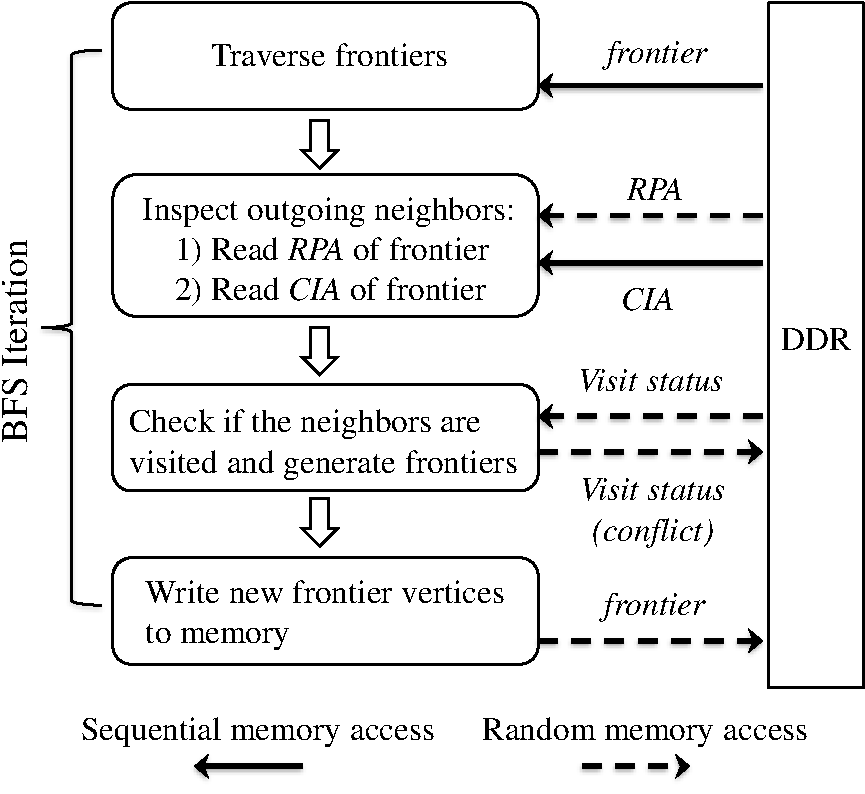
\includegraphics[width=0.7\linewidth]{base-bfs}}
    \caption{Baseline pipelined BFS}
\label{fig:base-bfs}
\vspace{-1em}
\end{figure}



\section{DNN Acceleration Fault Analysis Platform and Fault Classification}
\label{sec:fault-analysis}
\subsection{Fault Analysis Platform}
To conduct systematic analysis of faults on a DNN acceleration 
system, we build a fault analysis platform on Xilinx Zynq (ARM-FPGA) 
as shown in Figure \ref{fig:fault-analysis-overview}. It has a 
typical neural network accelerator implemented on FPGA. The accelerator 
is attached to the ARM processor in Zynq with AXI bus. Typically, the ARM processor 
can set up the neural network parameters, allocate specific memory 
space for bias/instruction/input/output/weight data 
and communicate with the DNN accelerator through shared memory. 
The ARM processor runs embedding Linux and can invoke the 
DNN accelerator through driver, providing a typical neural 
network acceleration system.

\begin{figure}
    \center{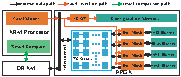
\includegraphics[width=0.99\linewidth]{system-overview}}
    \caption{Overview of the fault analysis system}
\vspace{-0.5em}
\label{fig:fault-analysis-overview}
\end{figure}

On top of the baseline FPGA-based neural network acceleration system, 
we also need a fault injection module as shown in 
Figure \ref{fig:fault-analyis-overview}. The fault injection data path 
is marked with orange arrows. It is implemented on both the ARM processor 
and FPGA. On the ARM processor part, it defines both the fault models 
such as bit-flip, stuck-at-0, and stuck-at-1, and the fault distribution 
models which determine the locations of the faults to be injected. Then it
generates the errors to be injected. On the FPGA part, the generated errors 
are sent to the FPGA from an AXI port accordingly. While errors in FPGAs are mainly 
located on the four different memory types including configuration memory, 
block memory, distributed memory and Flip-Flops. Currently, we randomly 
inject persistent errors to the first three memory types. Flip-Flops that 
get updated frequently are not handled in this work. 

For FPGA configuration memory, we take advantage of Xilinx ICAP 
port \cite{UG953}, which allows user logic to access configuration 
memory, to inject errors. While Xilinx FPGA bitstream is organized 
as frames and each frame includes configuration bits of a block of 
FPGA, we randomly choose the frame and the number of bits for each 
bit error injection. The error can be located at any place of the 
FPGA configuration memory including the regions that are not utilized.
When the position of an error is determined, we read the whole frame 
out of the configuration memory via AXI port of AXI-HWICAP \cite{PG134}, 
change the victim bit in the frame, and write it back to the configuration 
memory \cite{UG470}. This is done before the fault analysis, but it is also 
possible to do it at run-time.

For the block RAM and distributed memory, we develop an error injection 
mask (Err. Mask) which can be added to an on-chip memory block without 
changing the memory interface nor the pipelining. Meanwhile, it has an 
AXI slace port allowing ARM processor to flip a bit of any data in the 
memory block during reading. Figure \ref{fig:error-mask} shows the design 
of the error mask. Basically, it has a set of address and mask registers 
that can be configured using the attached AXI port. The addresses in 
the registers represent the position of errors to be injected while 
the corresponding masks keep the exact error bits. Whenever there is 
a read request coming to the block RAM, the read address will be compared 
with all the addresses in the registers. when there is an address match, 
the data read from the block RAM will be XORed with the mask.
Then the result will be used as the output of the block RAM 
affected by injected errors. The registers in the error mask 
can be configured in advance or at run-time. 

\begin{figure}
    \center{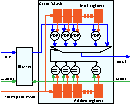
\includegraphics[width=0.7\linewidth]{error-mask}}
    \caption{Error mask for fault injection to on-chip memory}
\vspace{-0.5em}
\label{fig:error-mask}
\end{figure}

Another important part of the fault analysis platform is the result 
collection and comparison. We have the output of neural networks 
stored in the shared DRAM, which can be easily accessed on the ARM processor 
and compared to the pre-calculated golden reference. In addition, the computing 
results produced in the intermediate layers can also be compared.
The result comparison is mainly performed on the ARM processor and can be 
easily utilized for further analysis by high-level application designers.

\subsection{System fault classification}
Prior fault analysis works usually focus on computing errors of the neural networks 
and the incurred prediction accuracy loss. We argue that the consequences 
of hardware faults on a DNN acceleration system vary and should be classified 
into more categories. Table \ref{tab:classification} shows the proposed classification.
From the perspective of a system, the consequences caused by hardware faults 
roughly include system exception and accuracy degradation. System exception 
indicates that the neural network execution behaves abnormally, 
which may be stalled without returning or returns too fast or too slow.
Basically, we define them as system stall and abnormal runtime.
For the accuracy degradation, we
further classified into two cases including system stall 
and abnormal runtime.i

\begin{table}
    \centering
    \caption{Caption}
    \label{tab:classification}
    \begin{tabular}{c|cccc}
    \hline
      \multirow{2}{*}{system exception} & system stall\\
      \cline{2-2}
      & abnormal runtime\\
      \cline{1-2}
      \multirow{3}{*}{Accuracy degradation} &$$L0$\\
      \cline{2-2}
      & ... \\
      \cline{2-2}
      &$L_{k}$\\
      \cline{1-2}
      \hline
    \end{tabular}
\end{table}

We chose Neural Networks in four different application 
scenarios and try to analyze the differences of error 
tolerance in different application scenarios and networks. 
The four network applications include ResNet network for 
image classification, YOLO system for target detection, 
LSTM network for voice classification, and DCGAN network 
for image generation. We will evaluate their fault 
tolerance from accuracy and output consistency.

Neural Network accelerators injected with hardware errors 
may produce unexpected conditions. We define the system 
halt situation, which refers to a serious error in the 
system, or working improperly. such as unable to read and 
write registers, timeout, abnormal short runtime, etc. When 
the system halts, we need to reset the FPGA and restart the 
system. System halt situations are considered the result of 
errors in the evaluation of network accuracy and are listed 
separately in the output consistency.

Network accuracy refers to the overall accuracy of the 
network when performing corresponding tasks, such as the 
accuracy of 20,000 image recognition. When there are errors 
in the operation, the accuracy of the network will show a 
downward trend. For classification networks including 
ResNet and LSTM, top-5 accuracy is used to evaluate their 
accuracy, and for the YOLO system, mAP is adopted.

Output consistency is the difference between the result of 
running with errors injected and the result of normal 
running. We ran the corresponding data set when no errors 
are injected into each network at first, and defined the 
results as standard output. The results of Neural Networks 
prediction injected with errors are divided into two 
categories: result with deviation and result match. Result 
with deviation refers to system works properly with output 
differently from standard output. Result match means that 
the system works properly and the outputs are still 
standard output.

For the result with deviation case, we define its deviation 
quantitatively and further subdivide the result. Due to the 
different application functions of each network, the 
evaluation criteria of deviation are also different. For 
YOLO system, the result is the target detection bounding 
box, and when the detection result does not match the 
standard output in object type, it is defined as detection 
result error. When the result target type is consistent, 
the error is defined as the intersection area of the error 
output and the standard output divided by the area of the 
union. Target types not match for one single level, the two 
do not overlap with each other for one level, and then each 
20\% is divided into one level. For ResNet and LSTM, the 
outputs are top-5 labels. When the error output is not 
completely consistent with the standard output, the number 
of elements in the intersection of the two is taken, and 
divide the levels refer to the number. For DCGAN, we used 
the universal SSIM standard, and divided it into six levels 
according to the actual visual effects: 0~10\%, almost 
impossible to recognize; 10~20\%, barely visible; 20~50\%, 
with large deformation or distortion; 50~80\% with partial 
deformation or distortion; 80~90\%, small deformation or 
distortion can be seen; 90~100\%, almost no deformation or 
distortion is visible.

\section{Experiment} \label{sec:experiment}
We seek to understand the influence of persistent errors on 
FPGA-based neural network acceleration system. Particularly, 
we try to analyze the influence from a system point of view
and figure out the underlying reasons for severe system problems 
such as system stall and dramatic prediction accuracy loss. 

\subsection{Device and Environment}
Xilinx Zynq-7000 SoC ZC706 Evaluation Board will be used in 
the experiments’ hardware implementation. It has 
appropriate hardware resources and is easy to develop and 
use. The hardware design and Bitstream file compilation 
were completed using the upper computer with Intel Core 
i7-6700 processor and 2x8GB DDR4 2400MHz memory. The system 
environment used was Ubuntu 16.04 LTS version, and Xilinx 
Vivado Design Suite and Xilinx Software Development Kits 
version 2017.4.

The hardware resource utilization of the error analysis 
platform implementation on ZC706 is shown in Table \ref{tab:utilization report}.

The four models cover a broad range of applications.
Yolo represent a typical neural network model for object detection \cite{redmon2016yolo9000}, 
Resent is a widely adopted neural network model for classification \cite{He_2016_CVPR}, 
LSTM is the mostly used neural network model for audio classification 
tasks \cite{sak2014long}, and DCGAN stands for a typical neural network model for 
generative tasks \cite{radford2015unsupervised}. 

Despite the widespread adoption of deep learning 
neural network on various applications, it is particularly 
successful in four categories of tasks including object detection, 
object classification, voice recognition and style transfer.
Among a great number of neural network models,
Yolo, Resnet, LSTM and DCGAN are four typical neural networks 
that are comprehensively explored to handle the four computing 
tasks respectively. 

\begin{table}
    \centering
    \caption{Utilization Report of Fault Analysis Platform}
    \label{tab:utilization report}
    \begin{tabular}{cccc}
        \toprule
        Resource & Utilization & Available & Utilization Percentage \\
        \midrule
            LUT & 122618 & 218600 & 56.09\% \\
            LUTRAM & 185 & 70400 & 0.26\% \\
            FF & 84641 & 437200 & 19.36\% \\
            BRAM & 203 & 545 & 37.25\% \\
            DSP & 297 & 900 & 33\% \\
            MMCM & 1 & 8 & 12.5\% \\
        \bottomrule
    \end{tabular}
\vspace{-1em}
\end{table}

\subsection{Overview}
We hope to explore the possible consequences of errors, the 
fault-tolerant ability of different applications and the 
influence of different error locations of accelerators, 
which can provide meaningful references for the subsequent 
network optimization and the fault-tolerant design of 
accelerators.

We conducted five sets of experiments, which explained the 
influence of single error on different networks, the 
difference of fault tolerance ability of different 
applications, the error classification of different 
applications, the influence of different accelerator units 
and whether the input data affected the error representation.


\subsection{Error Consequences and Coverage}
First, we conducted single-bit random error injection 
experiments for different applications, and conducted 
20,000 runs for each application, to analyze the proportion 
of single-bit random error shielded in the system and the 
possible influence of single-bit random error on the 
accelerator system. Figure \ref{fig:lab1-error-rate} shows the 
percentage of application errors caused by a single-bit 
random hardware error. In the experiment, we found that 
more than 90\% of the errors were masked by software or 
hardware. However, while most errors are masked without 
impact to the operation, a single-bit error can lead to 
serious exceptions, including system halt, serious 
deviation in results, and so on. In addition, LSTM network 
has a better fault tolerance performance than other three 
networks, and the proportion of the influence caused by 
single error of the other three networks is about 5~7 times 
that of LSTM. According to our analysis, this is because 
LSTM network is smaller than other networks and uses less 
storage and computing resources.

\begin{figure}
	\center{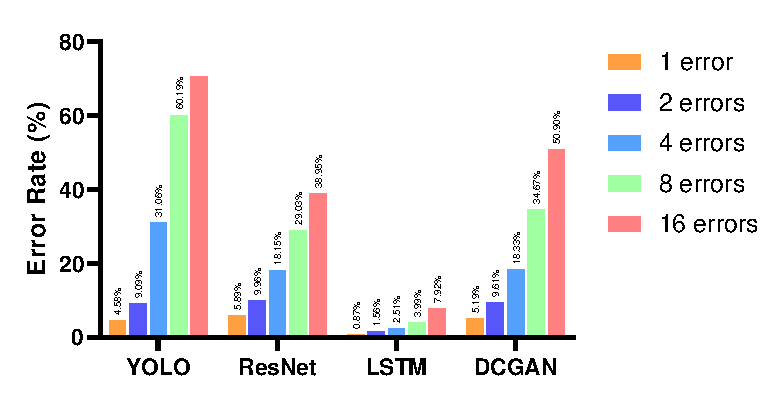
\includegraphics[width=0.9\linewidth]{lab1-error-rate}}
    \caption{Application error rate caused by single-bit random hardware error}
\label{fig:lab1-error-rate}
\vspace{-0.5em}
\end{figure}


\subsection{Effect of Error Number}
We completed a single run with errors injected number of 
powers of 2, with 20,000 runs for each network. In general, 
the proportion of system halt and result with deviation 
increases with the number of errors, and the accuracy of 
application decreases. Figure \ref{fig:lab2_2} show the proportion of 
system halt and result deviation, and Figure \ref{fig:lab2-network-accuracy} shows the 
accuracy of each network. We found that the influence of 
multiple errors on the accelerator was obvious and far 
beyond our expectation. The Neural Network accelerator is 
still vulnerable to errors. By the time we injected 16 
errors in a single run, the system halt rate was more than 
1\%, means it took more time to restore the system than to 
run it. From the perspective of network accuracy, take YOLO 
system as an example, its mAP decreases by 8.95\% when it 
runs with 16 errors, means the application function of the 
system is also seriously affected.

The result with deviation proportion of different networks 
appears differently with the increase of error number. When 
16 errors are injected, LSTM network still has a small 
result deviation proportion due to its small network 
structure. The proportion of YOLO system is very high, with 
about 70\% of the results showing errors. ResNet is 
relatively low, with only about 35\% result deviation. 
DCGAN network is in between, and about 50\% of the results 
have numerical errors. We believe that the result deviation 
may be related to the structure of the output. The output 
of YOLO system contains more information such as object 
type, location and size of bounding box, etc., and the 
output of ResNet is simple sorting, while the simple output 
is obviously less susceptible to errors.

\begin{figure}
	\center{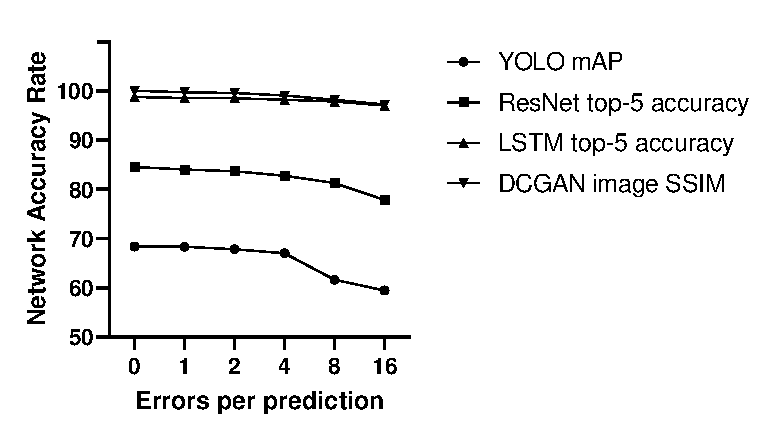
\includegraphics[width=0.85\linewidth]{lab2-network-accuracy}}
    \caption{Network accuracy versus error number}
\label{fig:lab2-network-accuracy}
\vspace{-0.5em}
\end{figure}

\begin{figure}
    \centering
    \subfigure[System halt]{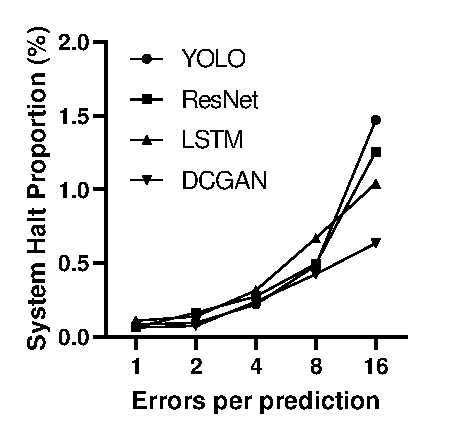
\includegraphics[width=0.45\linewidth]{lab2-system-halt}}
    \subfigure[Result with deviation]{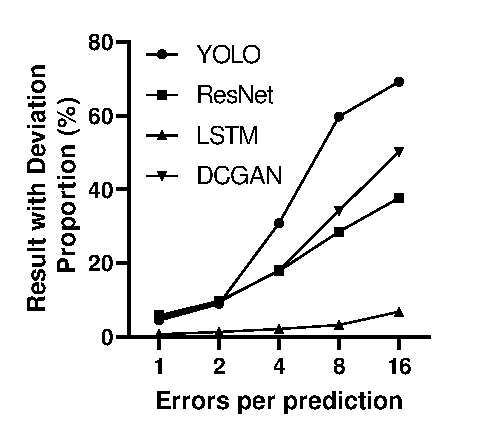
\includegraphics[width=0.45\linewidth]{lab2-result-with-deviation}}
    \caption{Abnormal situation proportion versus error number}
\label{fig:lab2_2}
\vspace{-0.5em}
\end{figure}


\subsection{Details of Result with Deviation}

\begin{figure*}
    \centering
    \subfigure[YOLO]{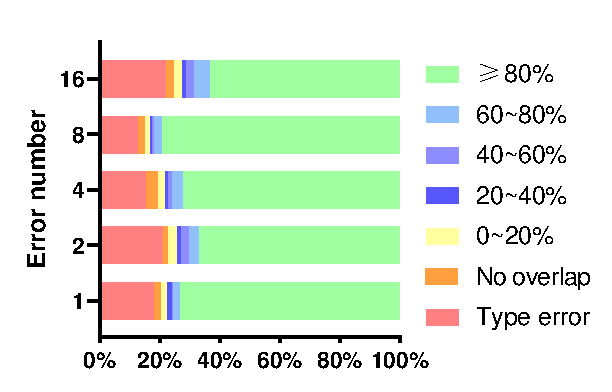
\includegraphics[height=0.12\textheight]{lab3-yolo}}
    \subfigure[ResNet]{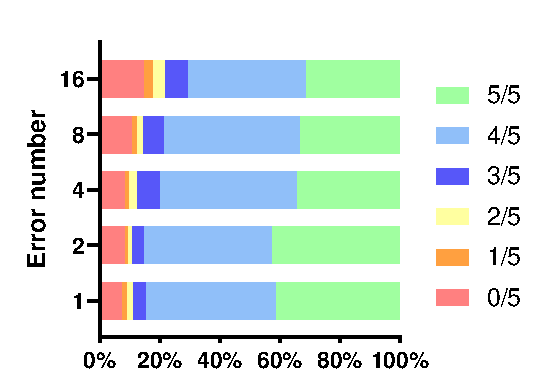
\includegraphics[height=0.12\textheight]{lab3-resnet}}
    \subfigure[LSTM]{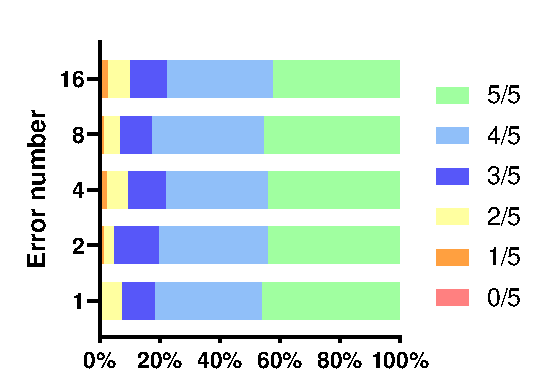
\includegraphics[height=0.12\textheight]{lab3-lstm}}
    \subfigure[DCGAN]{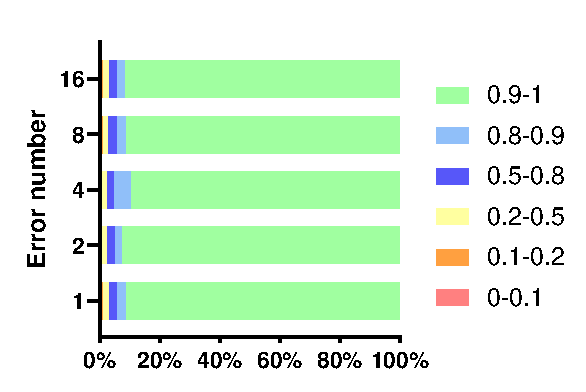
\includegraphics[height=0.12\textheight]{lab3-dcgan}}
\caption{Distribution of result with deviation situations}
\label{fig:lab3}
\vspace{-0.5em}
\end{figure*}

\begin{figure*}
    \centering
    \subfigure[YOLO]{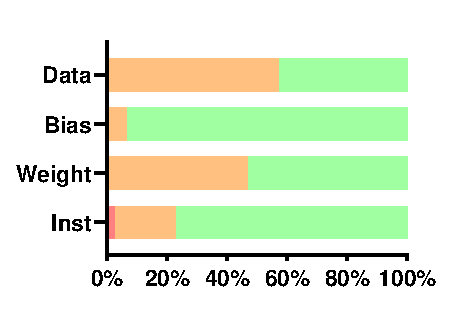
\includegraphics[height=0.10\textheight]{lab4-yolo}}
    \subfigure[ResNet]{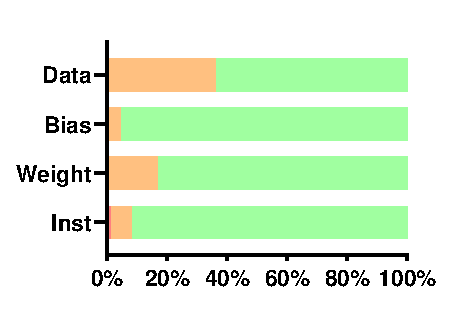
\includegraphics[height=0.10\textheight]{lab4-resnet}}
    \subfigure[LSTM]{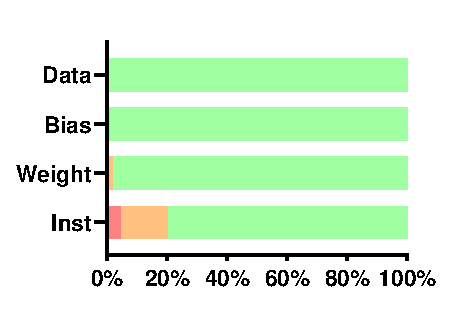
\includegraphics[height=0.10\textheight]{lab4-lstm}}
    \subfigure[DCGAN]{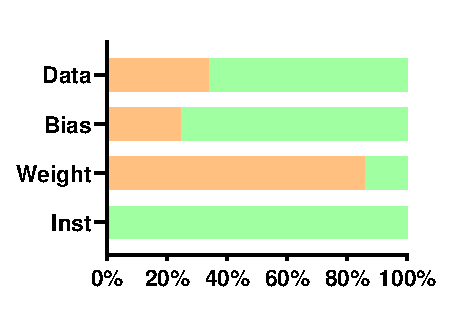
\includegraphics[height=0.10\textheight]{lab4-dcgan}}
    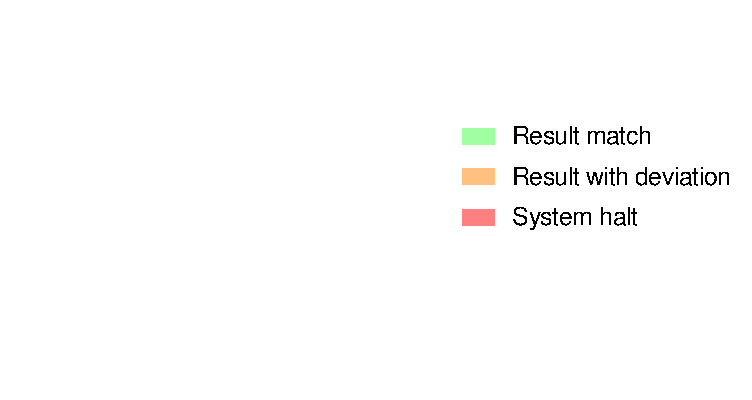
\includegraphics[height=0.10\textheight]{lab4-symbol}
\caption{Proportion of different error location}
\label{fig:lab4}
\vspace{-0.5em}
\end{figure*}

The results with errors are further classified and analyzed. In general, most of the errors are small, with a certain proportion of serious errors and relatively few moderate ones. We believe that most of the errors do not belong to the errors with global influence, but only affect one or several calculations. For example, a single value in the convolution kernel changes. Alternatively, a portion of the error is masked by subsequent calculations such as the max pooling layer. Some errors may have an impact on the control path or the reusable module, resulting in the accumulation of errors throughout the calculation; Or errors that cause serious deviations in the data, such as sign bit upset, can have serious consequences. Figure \ref{fig:lab3} shows the details of result distribution of result with deviation situations.

Specific to each network, about 70\% of the YOLO system's errors belong to the level of bounding box overlap ratio more than 80\%. The total of object type errors and non-overlapping boxes is about 20\%. The remaining 10\% or so is moderate errors. We think this is caused by the implementation of YOLO. YOLO divides the input images into a series of grid cells, and each grid cell is only responsible for one kind of object. Moreover, there is a binary judgment Pr(Object) whether there is a target or not in the confidence degree, which leads to more object type error cases. The bounding boxes that are given after object recognition based on relative wide and high are less sensitive.

More than 70\% of the errors in the ResNet and LSTM classification networks were small impact results of matching four or five items. We think this is because the output is SoftMax layer, which is less affected by the error, and the error is easy to be hidden when sorting, so the result only shows a small alter. However, with the increase of the number of errors, the proportion of serious errors of no matching item in ResNet results increased with the increase of the number of errors and exceeded 10\%. Serious errors cannot be hidden, and the networks fault tolerance for multiple errors is relatively limited.

The result of DCGAN is about 90\% of the results are small deviation level of more than 90\% of SSIM. Only a few of them have a large deviation. Combined with the image, in 90\% of the small deviation results compared with the standard output, basically no difference can be directly seen, and only a few large deviation results have serious distortion of the image. Considering that the output is picture information, these small deviations can be ignored without affecting the visual effect, we believe that DCGAN has relatively strong error tolerance.


\subsection{Effect of Error Location}
In this period, we conducted the experiment results of different error locations. We injected a single-bit random error into a designated location, and conducted multiple experiments to observe the performance of the network. By analyzing the influence of error in different locations on the accelerator, it can provide specific methods for the subsequent fault-tolerant design.

In general, the system is less affected by configuration memory errors, considering that the error injection of configuration memory is global, whose errors may not affect the system. Errors in configuration memory can cause system halt or result with deviation. Errors in BRAMs used for instruction buffer can cause system halt or result with deviation, while BRAMs used in other type buffers can only cause numerical deviations.

We focus on the analysis of the system halt situations caused by error in instruction buffer, which take about 20\% part of the system halt situations. Compared with the instruction before and after upset, the system halts caused by instruction errors includes three situations: instruction type changes, wrong instruction not defined, and the parameter in the operation is abnormal. Different instruction types of the original instruction are considered. Table \ref{tab:instruction change} and Table \ref{tab:original instruction type} shows the detail of instruction error. About 50\% of the system halt situations are caused by the error of DMA instructions. The abnormal access address or boundary violation caused by the abnormal parameters of DMA instruction will lead to the system halt. About 30\% are caused by AGU instruction errors, which result in abnormal in-chip control flow.

\begin{table}
    \centering
    \caption{Instruction change}
    \label{tab:instruction change}
    \begin{tabular}{cc}
        \toprule
            Situation & Percentage \\
        \midrule
            Error instruction undefined & 2.48\% \\
            Instruction type change & 7.45\% \\
            Abnormal parameter & 90.06\% \\
        \bottomrule
    \end{tabular}
\vspace{-1em}
\end{table}

\begin{table}
    \centering
    \caption{Original instruction type}
    \label{tab:original instruction type}
    \begin{tabular}{cc}
        \toprule
            type & Percentage \\
        \midrule
            DMA & 55.90\% \\
            AGU & 32.92\% \\
            others & 11.18\% \\
        \bottomrule
    \end{tabular}
\vspace{-1em}
\end{table}


The proportions of errors in instruction buffer led to system halt in ResNet, YOLO and LSTM, reached 1.15\%, 2.55\% and 4.25\% respectively, seriously affecting the proper application of the system. For result with deviation case, in the experiment of YOLO, about half of the result deviation situations caused by instruction buffer errors were serious object type errors. In the experiment of ResNet, a large number of mismatches were also caused. DCGAN network is limited by instruction errors, because the instruction sequence length of this network is very short, only 2\% of the instruction buffer is used, while the instruction sequence of other networks uses instruction buffer of 50\%\~{}80\%. Combined with the result with deviation and system halt case, we propose that instruction buffer needs to be strengthened in the fault-tolerant design.


Errors in the buffers used in data-flow, such as weights, data, and bias buffer, do not cause system halt, only may cause result deviations. In general, data and weights are more sensitive than bias. Taking YOLO system as an example, the proportion of result deviation caused by single error in weight, data and bias buffer is 48.75\%, 56.95\% and 6.35\% respectively. Horizontal comparison shows that each network has different sensitivity to different buffer errors, as shown in figure {}.


\subsection{Input-Related Error}
In the above experiments, we used different input data for 
experiments, and we verified the relationship between 
errors and input data in this set of experiments. We test 
different input data using the same error. Whether a 
hardware error causes an application error exists in two 
ways, depending on the input data or not. Errors unrelated 
to input data, fixed to cause system halt or result 
deviation, or be masked, that is, different input data will 
not influence the classification of the result. The other 
part of the errors is input data related, which can be 
shown as replacing different input data, result match 
situation and result with deviation situation both appear. 
In other words, different input data has different 
sensitivity to an input-related error. We believe that this 
is caused by structures which error affected. 
Input-unrelated errors may affect the control-flow of the 
system, the bus, etc. These structures are used in every 
operation, and the errors will not be masked by subsequent 
calculations. Input-related errors may affect the relevant 
data in the data-flow, and some errors may be masked in 
the subsequent calculation. Due to the large number of 
experiments, we only observed this phenomenon without 
further study on its proportion and distribution.



\section{Related Work} \label{sec:relatedwork}
Despite of the performance and power advantages, the design 
productivity of developing FPGA applications remains low 
due to the lengthy compilation and complex application-specific 
customization. And it has become the major obstacle 
that hinders the wide adoption of FPGAs as commodity computing devices. 
The community from both the industry and academia have developed 
many different methods from diverse angles to tackle the problem. 
These methods can be roughly classified into three categories. 
The first category mainly focuses on improving the low-level 
implementation tools. A number of approaches such as making 
quality/runtime trade-offs \cite{mulpuri2001runtime}, parallel 
compilation \cite{moctar2014parallel, goeders2011deterministic, altera-pc, 
xilinx-pc} and using hard-macro techniques \cite{lavin2013improving, 
korf2011automatic} have been explored from this angle. The second 
category mainly centers the HLS design flow while the third one 
primarily relies on the overlay concept. They later two categories 
will be detailed in the following sections.

\subsection{High-Level Synthesis} 
With many years of continuous endeavor, a number of tools have emerged as 
mature solutions for HLS \cite{VivadoHLS, Legup, zhang2008autopilot}. They typically 
allow designers to express hardware designs using high-level  
description languages such as C, C++ etc. and also enable evaluation of different 
design choices using pragmas or directives. Indeed, they significantly improve 
the design productivity compared to the conventional hardware design flow using 
hardware description languages. However, when considering the overall design 
productivity of developing hybrid software-gateware applications, HLS is 
only addressing part of the problem, as the lengthy low-level compilation 
including synthesis, mapping, placing and routing remains a bottleneck for 
an application designer \cite{ROB2014, capalija2014tile}.

Customizing the generated hardware specifically to an user 
application is also time-consuming for designers and thus critical to the design 
productivity. A number of algorithms such as generic algorithms 
relied on local-search techniques \cite{schafer2009adaptive, 
sengupta1997genetic}, learning-based methods \cite{onlinecustomization, 
carrion2012machine}, divide and conquer algorithm \cite{DCcustomization} 
and a calibration free algorithm \cite{RCcustomization} etc. have been developed 
to perform the DSE on top of HLS tools. The algorithms can efficiently help automate the 
customization or DSE process. However, the algorithms must rely on HLS tools 
to estimate the implementation information such as implementation frequency, 
overhead or power for the corresponding customization. While the hardware generated 
can be irregular and may vary dramatically, thus the accuracy of the estimation 
especially on implementation frequency and power can be rather limited, which may
fail to optimize an HW/SW co-design problem.  

\subsection{Overlay Architectures}
Overlay architecture which is a virtual intermediate architecture overlaid on 
top of off-the-shelf FPGA is increasingly applied as a way to address the 
productivity challenge. 

Various overlays with diverse configuration granularities and flexibility 
ranging from virtual FPGAs \cite{Grant2011Malibu, ZUMA2012}, 
array-of-FUs \cite{mesh-FUs,ferreira2011fpga}, soft 
CGRA \cite{kissler2006dynamically, scgra-orig}, soft GPU \cite{Guppy2012GPU-Like}, 
vector processors\cite{Yiannacouras2009FPS, MXP2013} to 
configurable processors or multi-core processors \cite{unnikrishnan2009application, 
MARC2010, Yiannacouras2007Exploration, Capalija2009coarse-grain, OCTAVO2012, iDEA2012} 
have been developed over the years. SCGRA overlay provides unique 
advantages on compromising hardware implementation 
and performance for compute intensive nested loops as demonstrated 
by numerous ASIC CGRAs \cite{tessier2001reconfigurable, compton2002reconfigurable}.
Most importantly, it allows both rapid compilation by taking advantage of 
the overlays' tiling structure \cite{ROB2014} and efficient bitstream 
reuse within the design iterations of an application \cite{scgra-orig}, 
thus it is particularly promising for high productivity nested loop acceleration.

Despite of the promising potential, a complete automatic customization 
framework that enables application-specific optimization is still highly 
anticipated for the sake of design productivity and performance. 
The authors in \cite{colinheart} developed an SCGRA topology customization method 
using genetic algorithm and showed the potential benefits of the SCGRA 
overlay customization. However, the rest system design parameters such as 
on chip buffer size, loop unrolling factor etc. are not covered. 

Indeed, SCGRA overlays have many similarities in terms of array structure 
and scheduling algorithm with ASIC CGRAs. Nevertheless, ASIC CGRAs emphasize 
more on configuration capability and limited customization is allowed due 
to the overhead constraints \cite{zhou2014application, miniskar2014retargetable} 
while SCGRA overlays allow more intensive architectural customization 
because of the FPGA's inherent programmability. Moreover, hardware resources such as 
DSP blocks and RAM blocks available on FPGAs are discrete, which results in different 
design constraints for SCGRA overlay customization as well. 

By utilizing the SCGRA overlay as the backbone of the FPGA accelerator, 
a complete nested loop acceleration framework 
targeting CPU-FPGA system is developed. It supports intensive application-specific
customization including the overlay architectural customization, 
the compilation customization and communication interface customization 
for various design goals. When the customized design parameters are determined, 
corresponding hardware accelerator and software can be compiled to the target 
CPU-FPGA system rapidly eventually providing a push-button solution for a nested loop 
acceleration. 



\section{Conclusion} \label{sec:Conclusion}
In this work, we propose to replace the forward computing on GPPs with accelerator 
computing during training and have both the computing 
errors and the application data learned in the neural network models. 
In addition, we opt to protect critical neural layers to reduce the negative 
influence of computing errors.  
With the proposed resilient neural network training, 
the prediction accuracy of the retrained neural network models improves significantly 
when computing errors appear. 


%\appendix
%\section{Acknowledgement}

%\begin{acks}
%  The authors would like to thank Sam Ho for providing the suggestions on
%  HLS design debugging and optimization as well as the SDAccel usage. 

%\end{acks}




%\section*{Acknowledgment}
    % acknowledgment content



% trigger a \newpage just before the given reference
% number - used to balance the columns on the last page
% adjust value as needed - may need to be readjusted if
% the document is modified later
%\IEEEtriggeratref{8}
% The "triggered" command can be changed if desired:
%\IEEEtriggercmd{\enlargethispage{-5in}}


% references section

% can use a bibliography generated by BibTeX as a .bbl file
% BibTeX documentation can be easily obtained at:
% http://mirror.ctan.org/biblio/bibtex/contrib/doc/
% The IEEEtran BibTeX style support page is at:
% http://www.michaelshell.org/tex/ieeetran/bibtex/
%\bibliographystyle{IEEEtran}
% argument is your BibTeX string definitions and bibliography database(s)
%\bibliography{IEEEabrv,../bib/paper}
%
% <OR> manually copy in the resultant .bbl file
% set second argument of \begin to the number of references
% (used to reserve space for the reference number labels box)

%\begin{thebibliography}{99}
%\bibitem{b1}
%G. Eason, B. Noble, and I. N. Sneddon, 
%``On certain integrals of Lipschitz-Hankel type involving products of Bessel functions,'' 
%Phil. Trans. Roy. Soc. London, vol. A247, pp. 529--551, April 1955.
%\bibitem{b2} 
%J. Clerk Maxwell, 
%A Treatise on Electricity and Magnetism, 3rd ed., vol. 2. 
%Oxford: Clarendon, 1892, pp.68--73.
%\bibitem{IEEEhowto:kopka}
%H.~Kopka and P.~W. Daly, \emph{A Guide to \LaTeX}, 3rd~ed.\hskip 1em plus
%  0.5em minus 0.4em\relax Harlow, England: Addison-Wesley, 1999.
%\end{thebibliography}


\bibliographystyle{IEEEtran}
\bibliography{refs}


\end{document}
